% $•$% !TeX root = macro_PS6_case.tex

\documentclass[12pt,oneside,reqno]{amsart}
    % \documentclass[]{article}
\usepackage{amssymb}
\usepackage{amsmath}
\usepackage{enumitem}
\usepackage{bm}
\usepackage{cases}
\usepackage{changepage}
\usepackage{amsfonts}
\usepackage{centernot}
\usepackage{graphicx}
\usepackage{float}
\usepackage{hyperref} % to restart section numbers for different parts
\usepackage{physics} % to get partial derivatives 
\usepackage{xcolor}
\usepackage[a4paper, total={6in, 8in}]{geometry}
\usepackage{listings} % to input code
       \lstset{backgroundcolor = \color{white},
               % frame = single,
               %keywordstyle=\color{blue}
               }
\usepackage{etoolbox}
% \patchcmd{<cmd>}{<search>}{<replace>}{<success>}{<failure>}
\patchcmd{\section}{\centering}{}{}{}
    % made section title not centered 
\let\flushleftsection\section% Copy updated non-centered definition of \section
\newcommand{\sectionscenter}{\let\section\centeredsection}% Switch to centered \section
\newcommand{\sectionsleft}{\let\section\flushleftsection}% Switch to flush left \section

\setlength{\parindent}{0em} % no automatic indents

%opening
\title{Econ 714 Quarter 1: Problem set 3 }
\author{Emily Case}

% command for blank footnote 
\newcommand\blfootnote[1]{%
	\begingroup
	\renewcommand\thefootnote{}\footnote{#1}%
	\addtocounter{footnote}{-1}%
	\endgroup
}

\newcount\colveccount
\newcommand*\colvec[1]{
	\global\colveccount#1
	\begin{pmatrix}
		\colvecnext
	}
	\def\colvecnext#1{
		#1
		\global\advance\colveccount-1
		\ifnum\colveccount>0
		\\
		\expandafter\colvecnext
		\else
	\end{pmatrix}
	\fi
}

\newcommand{\R}{\mathbb{R}}
\newcommand{\E}{\mathbb{E}}
\newcommand{\co}[2]{c_{#1}^{#2}} % makes subscript and superscript easier for consumption
\newcommand{\spa}{\text{ }}
\newcommand{\lnl}{\ell_n} % log likelihood function
\newcommand{\bxn}{\bar{X}_n}
\newcommand{\lag}{\mathcal{L}}
\newcommand{\sumin}{\sum\limits_{i=1}^n} % generic sumation 1 to n
\newcommand{\sumti}{\sum\limits_{t=0}^\infty} % sum - infinite horizon
\newcommand{\pin}{\Pi_{i=1}^n}
\newcommand{\argmax}{\text{arg}\max}
\newcommand{\fix} [1] {\textbf{\textcolor{blue}{#1}}} % use this to more clearly note in problem set pdf where things need to be changed. 
% end preamble

\renewcommand*{\thesection}{\arabic{section}}
\newcommand\numberthis{\addtocounter{equation}{1}\tag{\theequation}} % for equation numbering within align*

\begin{document}
	
	\maketitle
	
	\blfootnote{I worked on this Problem set with Sarah Bass, Michael Nattinger, Alex von Hafften, Hanna Han, and Danny Edgel.} 


%%%%%%%%%%%%%%%%%%%%%%%%%%%%%%%%%%%%%%%%%%%%%%%%%%%%%%%%%%
This problem asks you to update the CKM (2007) wedge accounting using more recent data.You are encouraged to use Matlab for the computations.  Consider a standard RBC modelwith the CRRA preferences

\begin{align*}
& \E_0 \sumti \beta^t U(C_t,L_t), 
& U(C,L) = \frac{C^{1-\sigma}-1}{1-\sigma} - \frac{L^{1+\phi}}{1+\phi}
\end{align*}

a  Cobb-Douglas  production  function $Y_t=A_tK^{\alpha}_tL^{1-\alpha}_t$,  a  standard  capital  law  of  motion $K_{t+1}= (1-\delta)K_t+I_t$, and four wedges $\tau_t=\{a_t,g_t,\tau_{L,t},\tau{I,t}$.  Each wedge $\tau_{it}$ follows an AR(1) process $\tau_{it}=\rho_i \tau_{it-1}+\epsilon_{it}$ with innovations $\epsilon_{it}$ potentially correlated across $i$.  One period corresponds to a quarter.

%%% 1 %%% no action required
\section{Download quarterly data for real seasonally adjusted consumption, employment, andoutput in the U.S. from 1980–2020 from FRED database.  The series for capital are notreadily available, but can be constructed using the “perpetual inventory method”.  To this end, download the series for (real seasonally adjusted) investment from 1950-2020.}



%%% 2 %%% no action required 
\section{Convert all variables into logs and de-trend using the Hodrick-Prescott filter.}
See matlab code. 



\pagebreak
%%% 3 %%% 
\section{Assume that capital was at the steady-state level in 1950 and the rate of depreciation is $\delta= 0.025$ and use the linearized capital law of motion and the series for investment to estimate the capital stock (in log deviations) in 1980-2020.  Justify this approach.}
First, log-linearize the capital law of motion:
    \footnote{Note that in the steady state, $\delta\bar{K} =\bar{I} $.}
\begin{align*}
k_{t+1} & = (1-\delta)\frac{\bar{K}}{\bar{K}} k_t + \frac{\bar{I}}{\bar{K}}i_t 
\\
k_{t+1} & = (1-\delta)k_t +\delta i_t
\end{align*}

Using this formula, and knowing that we have data for investment back to 1950, consider $t+1=1980Q1$ and iterate it:
\begin{align*}
k_{1980Q1} & = (1-\delta)k_{1979Q4}+\delta i_{1979Q4}
\\
& = (1-\delta)[(1-\delta)k_{1979Q3} +\delta i_{1979Q3}
    ]+\delta i_{1979Q4}
    \\
& = (1-\delta)^2k_{1979Q3} +\delta (1-\delta)i_{1979Q3}
    +\delta i_{1979Q4} 
    \\
& = (1-\delta)^2[(1-\delta)k_{1979Q2} +\delta 
    i_{1979Q2}]
    +\delta (1-\delta)i_{1979Q3}
    +\delta i_{1979Q4} 
    \\
& = (1-\delta)^3k_{1979Q2} +\delta (1-\delta)i_{1979Q2}
    +\delta (1-\delta)i_{1979Q3}
    +\delta i_{1979Q4} 
    \\
& = (1-\delta)^Tk_{1950Q1} 
    + \delta\sum_{j = 0}^{T-1}(1-\delta)^j i_{1979Q4-j}
\end{align*}
where $T$ is the number of periods between 1950Q1 and 1980Q1. In general, we have the decomposed law of motion as:
\[k_{t+1} = (1-\delta)^Tk_{t-T} 
    + \delta\sum_{j = 0}^{T-1}(1-\delta)^j i_{t-j} \]
Recall that capital has small deviations and does not jump in response to shocks, so $k_t$ will be small. Also, $(1-\delta)^T$ is also very small. This means that the capital in the first quarter of our data (1950Q1) does not really contribute much to our capital level in 1980. It becomes less and less important as time progresses. Because of this, we approximate it to be zero, and determine tomorrow's capital to be determined by the history of investment.
\[k_{t+1} = 
    + \delta\sum_{j = 0}^{T-1}(1-\delta)^j i_{t-j} \]


\pagebreak
%%% 4 %%%
\section{Linearize  the  equilibrium  conditions.   Assuming $\beta=  0.99$, $\alpha=  1/3$, $\sigma=  1,\;\phi=  1,\; \tau_L=\tau_I= 0$ in steady state,  and the steady-state share of government spendings in GDP equal 1/3,  estimate $a_t,\;g_t$ and $\tau_{L,t}$ for 1980-2020.  Run the OLS regression for each of these wedges to compute their persistence parameters $\rho_i.$}
The equilibrium conditions are:\footnote{We derived these in class}
\begin{align}
Y_t & = A_tK_t^\alpha L_t^{1-\alpha} 
\label{production}
\\
Y_t & = C_t+I_t+G_t 
\label{marketcl}
\\
L_t^\phi C_t^\sigma & = (1-\tau_{L,t})A_t(1-\alpha)K_t^\alpha L_t^{-\alpha} 
\label{labor}
\\
C_t^{-\sigma} (1 + \tau_{I,t}) 
& = \beta \E_t \bigg[ C_{t+1}^{-\sigma} [ A_{t+1}\alpha K_{t+1}^{\alpha-1}L_{t+1}^{1-\alpha} +(1-\delta)(1+\tau_{I,t+1})]\bigg]
\label{euler}
\end{align}
Now, we log linearize. The first two equations are straight forward to do so:
\begin{align*}
y_t & = a_t +\alpha k_t + (1-\alpha) l_t 
\tag{\ref{production}*} \label{productionLL} \\
y_t & = \frac{\bar{C}}{\bar{Y}} c_t + \frac{\bar{I}}{\bar{Y}}i_t + \frac{\bar{G}}{\bar{Y}}g_t 
\tag{\ref{marketcl}*} \label{marketLL}
\end{align*}
Note that if we log linearize $\tau_i$, we get a problem because $\bar{\tau}_L=\bar{\tau}_I= 0$, so we only linearize them. Let $X_t = 1-\tau_{L,t}$, then 
$x_t = -\hat{\tau}_{L,t} $. Now we can log linearize the labor equation:
\begin{align*}
\phi l_t +\sigma c_t 
& = -\hat{\tau}_{L,t}  + a_t + \alpha k_t -\alpha l_t
\tag{\ref{labor}*} \label{laborLL}
\end{align*}
Now suppose $Z_t = 1+ \tau_{I,t}$, then $z_t = \hat{\tau}_{I,t}$. Finally, we can do the euler equation: 
\begin{align*}
\sigma(\E_t[c_{t+1}] -c_t) +\hat{\tau}_{I,t} 
& = \beta \E_t \big[ \alpha\bar{A}\bar{K}^{\alpha-1}\bar{L}^{1-\alpha}(a_{t+1}+(1-\alpha)(l_{t+1}-k_{t+1}))+(1-\delta)\hat{\tau}_{I,t+1}
\big]
\tag{\ref{euler}*} \label{eulerLL}
\end{align*}

Once calculating the steady state values\footnote{I do this in matlab}, we have everything we need to find $a_t,\; g_t,\; \hat{\tau}_{L,t}$. The persistence rho's are:\footnote{Note that rho I is from calculations later in the problem set}. 

\begin{table} [h]
\centering
\caption{}
\begin{tabular}{ll}
& rho \\ 
\hline 
a & 0.72622 \\ 
g & 0.85589 \\ 
tau L & 0.57029 \\ 
tau I & 0.45171 \\ 
\hline 
\end{tabular}
\end{table}

%%% 5 %%% 
\section{Write down a code that implements the Blanchard-Kahn method to solve the model. Use the values of parameters, including $\rho_a,\;\rho_g$ and $\rho_{\tau_L}$, obtained above, and assume $\rho{\tau_I}= 0$ for now.}
Note that we can decompose our system:
\begin{align*}
\E_t X_{t+1} = \E_t \colvec{2}{k_{t+1}}{c_{t+1}} 
& = AX_t +BZ_t
\\
\Rightarrow 
\E_t X_{t+1} & = Q\Lambda Q^{-1} X_t +BZ_t
\\
\Rightarrow
\E_t Y_{t+1} & = \Lambda Y_t + Q^{-1} B Z_t
\\
& = \Lambda Y_t + C Z_t
\end{align*}
where $Z_t$ is a column vector of the 4 wedges. Solving and decomposing this by hand is cumbersome, so my matlab code solves for A, B, decomposes, etc. When I find the eigenvalues in matlab, it is clear that one is greater than 1 and one is less than 1. WLOG suppose $\lambda_1>1$, then we can take a part of the system:
\begin{align*}
\E_t Y_{1,t+1} & = \lambda_1 Y_{1,t} + C_1 Z_t
\\
Y_{1,t} & = \lambda^{-1}\E_t Y_{1,t+1} -\lambda^{-1}C_1 Z_t
\end{align*}



%%% 6 %%%
\section{Solve the fixed-point problem to estimate $\tau_{I,t}$:  conjecture a value of $\rho_{\tau_I}$, solve numerically the model for consumption as a function of capital and wedges, use the estimated values of consumption and other wedges to infer the series of $\tau_{I,t}$, run AR(1) regression and estimate $\rho_{\tau_I}$, iterate until convergence.}
Note that 
\[Q^{-1} \colvec{2}{k_t}{c_t} = \Theta \colvec{4}{a_t}{g_t}{\hat{\tau}_{L,t}}{\hat{\tau}_{I,t}} \]
and we can multiply out and get the following formula for $\hat{\tau}_{I,t}$:
\[\hat{\tau}_{I,t} = \frac{1}{\Theta_4} \big[Q_{1,1} k_t+Q_{1,2}c_t -(\Theta_1a_t+\Theta_2 g_t +\Theta_3 \hat{\tau}_{L,t})\big]\]
So we can easily find $\hat{\tau}_{I,t}$ and also $\rho_{\tau_I}$. See matlab code. 


%%% 7 %%%
\section{Draw one large figure that shows dynamics of all wedges during the period.}
Now we have all of the wedges and can plot them. Note that 0 corresponds to 1980Q1. 
\begin{figure} [h]
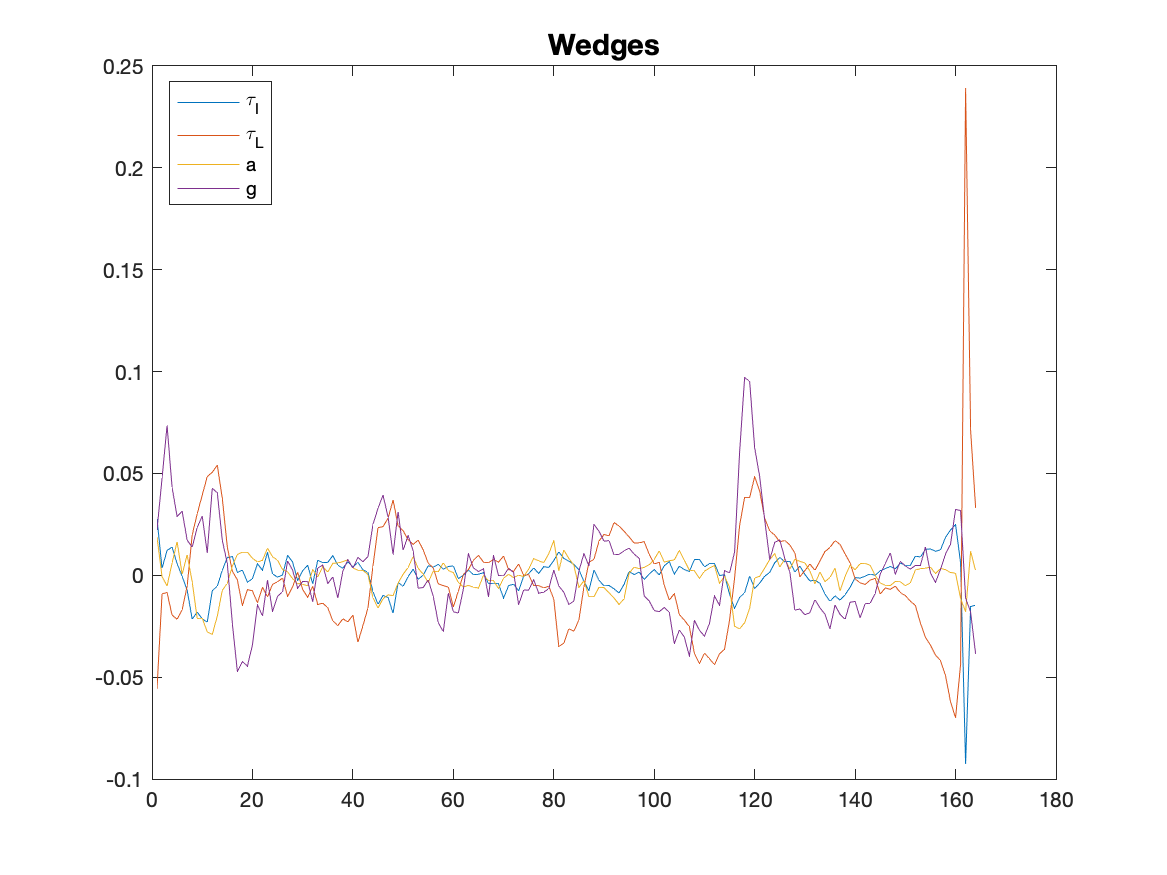
\includegraphics[scale=.7]{wedges}
\end{figure}


%%% 8 %%% 
\section{Solve the model separately for each wedge.  Show a figure with the actual GDP and the four counterfactual series of output.  Which wedge explains most of the contraction during the Great Recession of 2009?  during the Great Lockdown of 2020?  Explain.}

It seems from this that the wedge that influences GDP the most is technology (a), which makes sense as we are in a technological age. \\
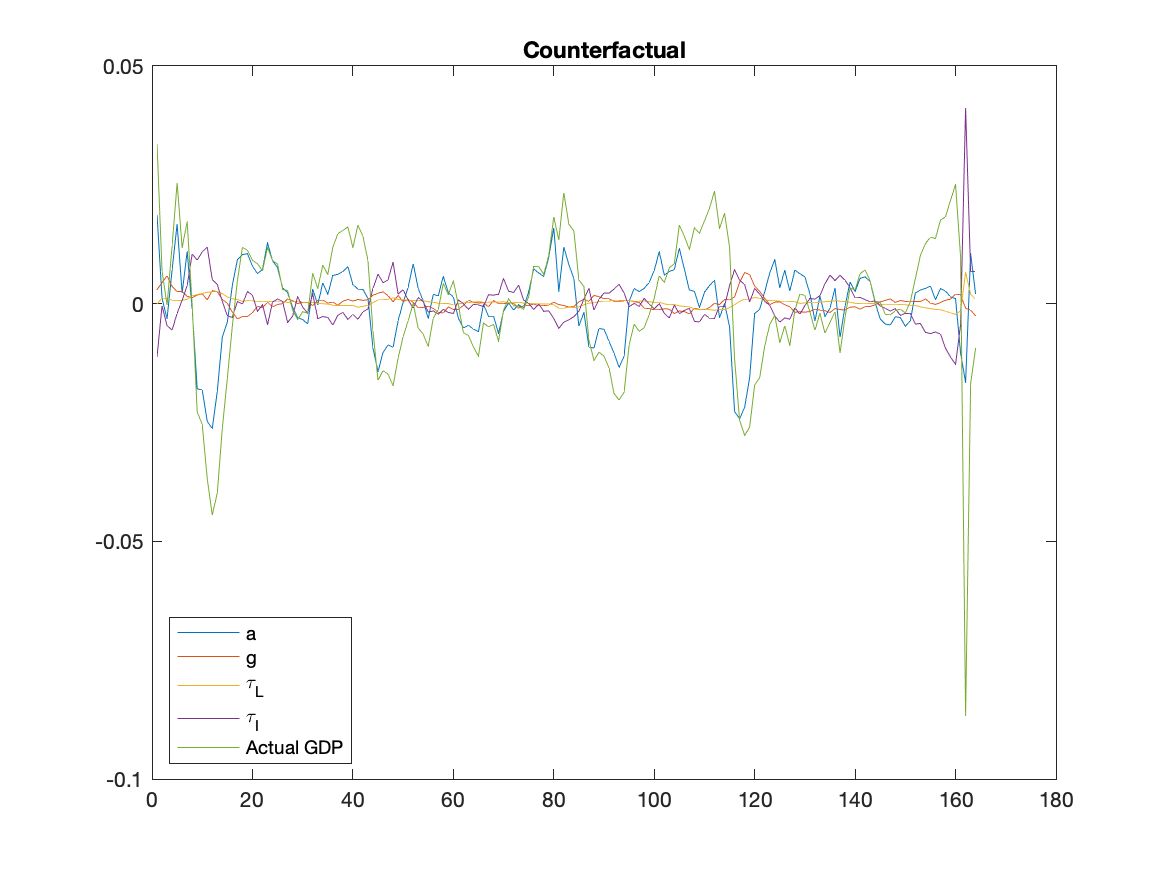
\includegraphics[scale=.7]{counterfact}

\end{document}
